%% This is an example first chapter.  You should put chapter/appendix that you
%% write into a separate file, and add a line \include{yourfilename} to
%% main.tex, where `yourfilename.tex' is the name of the chapter/appendix file.
%% You can process specific files by typing their names in at the 
%% \files=
%% prompt when you run the file main.tex through LaTeX.
\chapter{Introduction}

%% Chapter outline goes here
In this chapter, the construction of a fiber optic Doppler optical coherence microscopy system will be motivated. Additionally, the mathematical underpinnings of the system will be introduced, and recent related work will be discussed.

\section{Motivations for a fiber optic DOCM system}

\label{sec:intro}

The mammalian cochlea is capable of remarkable sensory perception. It can distinguish vibratory motion as small as the radius of a hydrogen atom and discriminate between up to 30 frequencies within a single semitone \cite{ghafarri}. However, the mechanics of motion in the inner ear remain poorly understood. The Micromechanics Group at the Research Laboratory of Electronics at MIT is analyzing motion in the cochlea in order to more fully understand what enables these remarkable sensory capabilities.

\begin{figure}[h!]
  \centering
    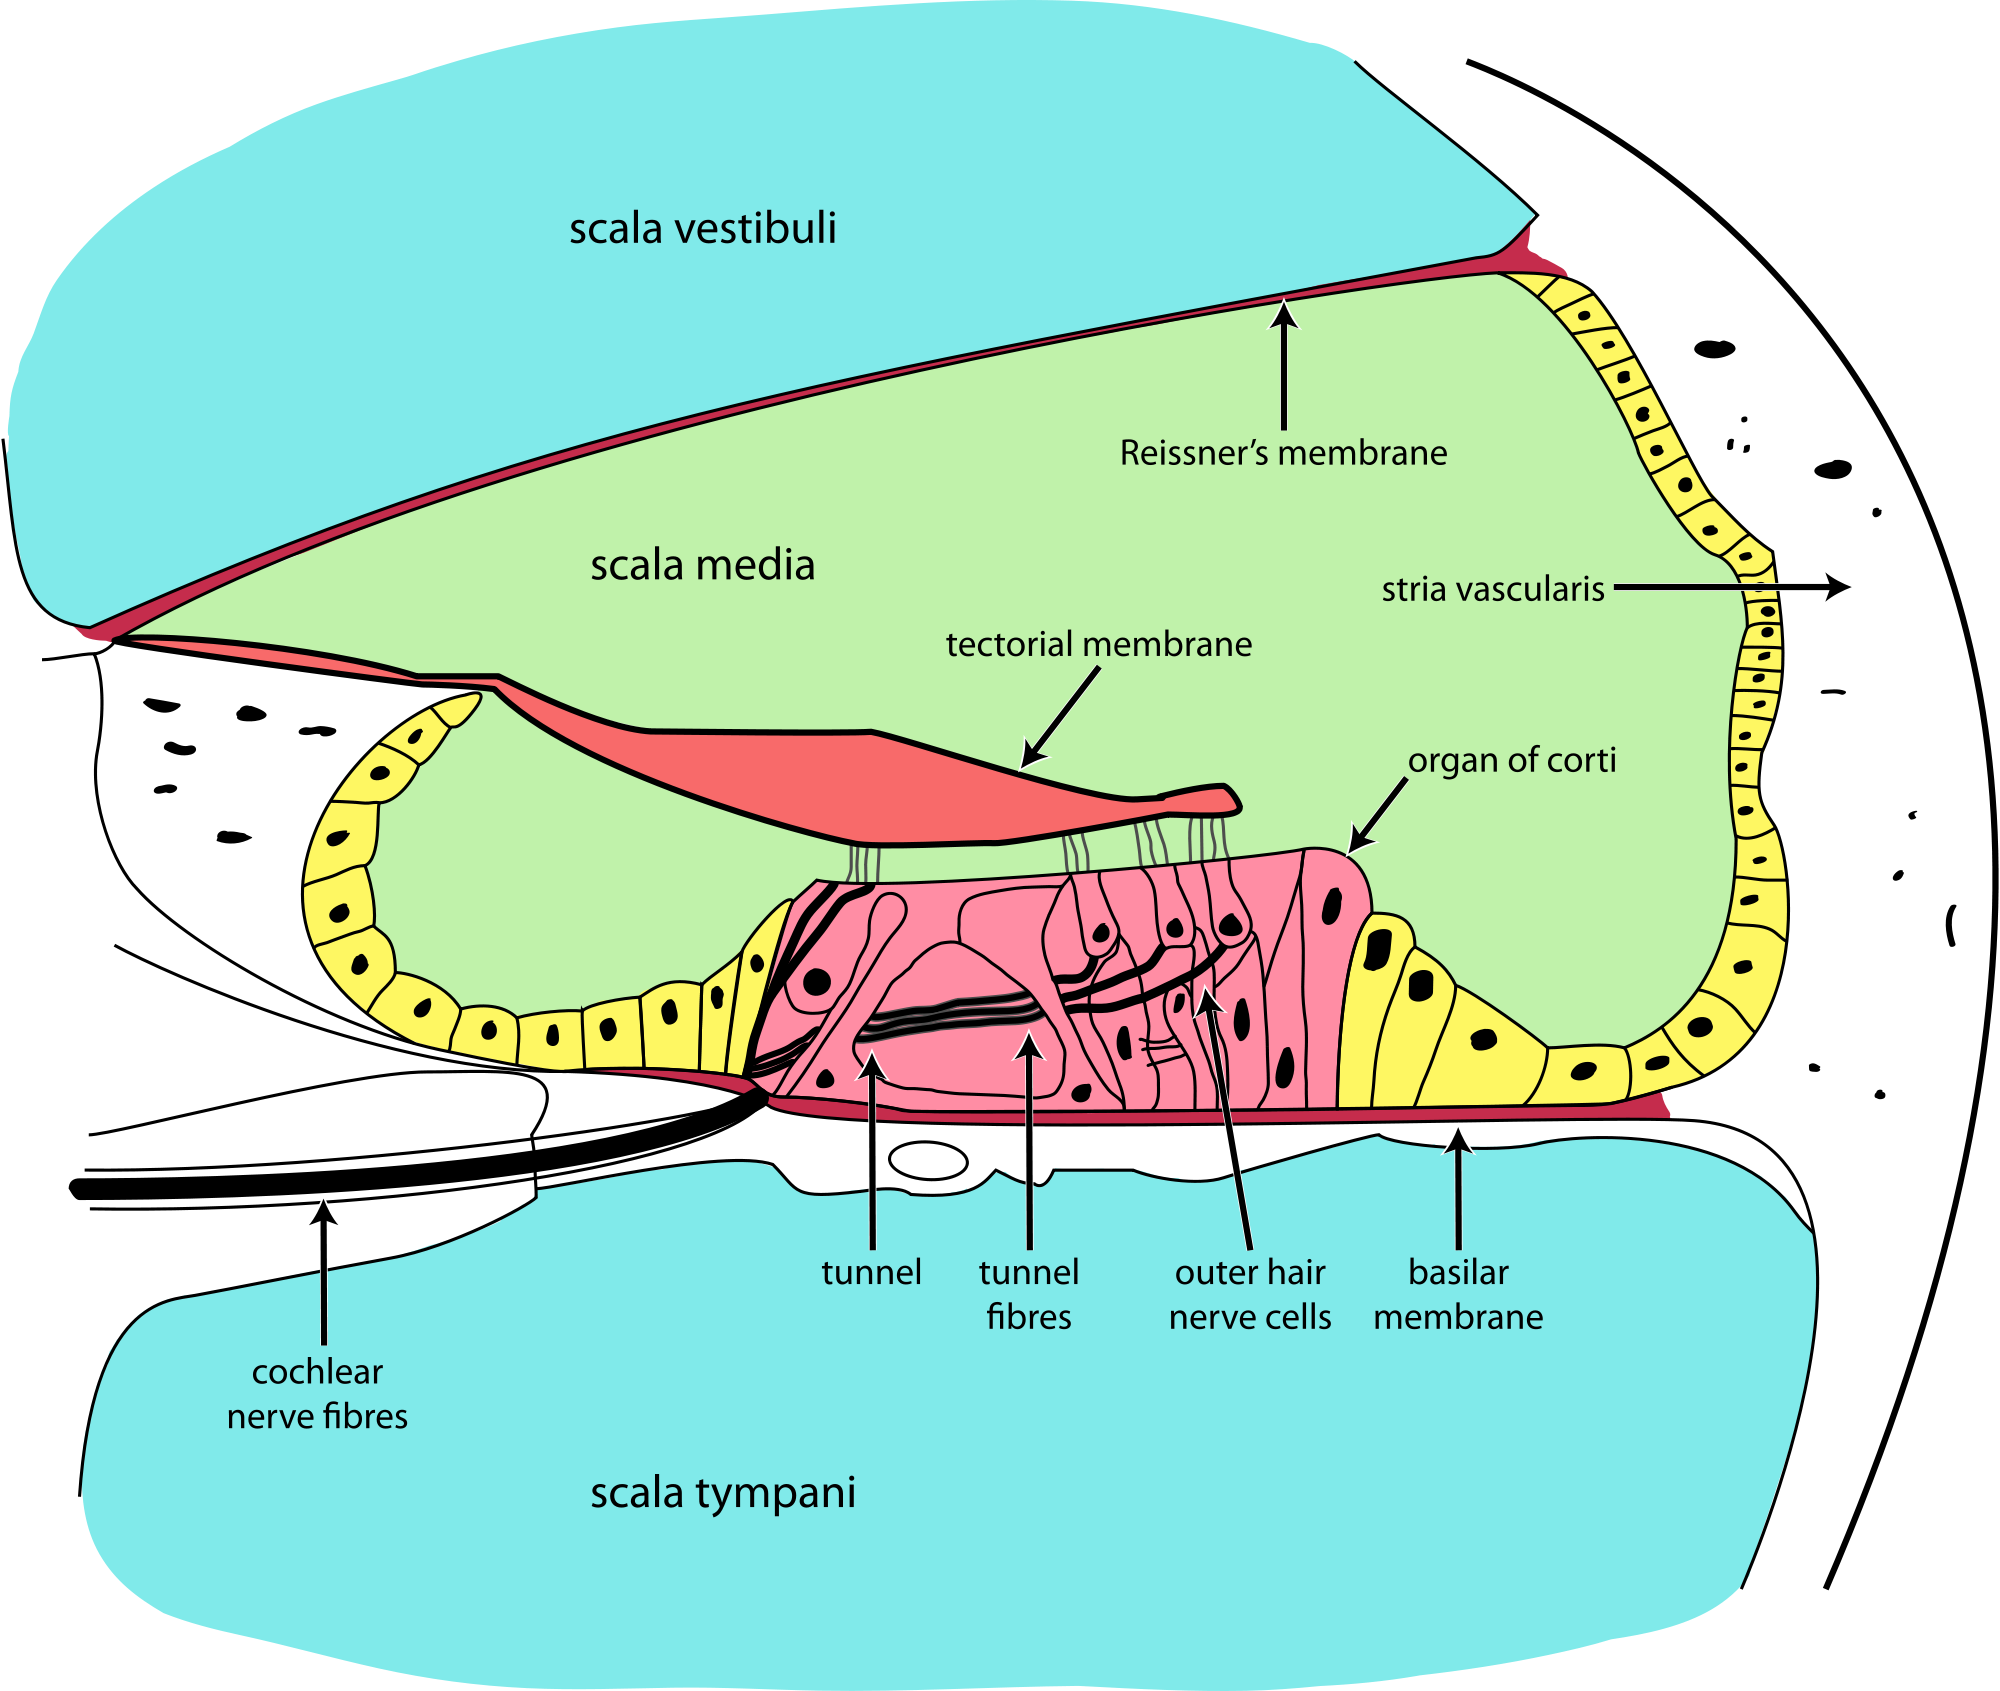
\includegraphics[width=0.85\textwidth]{Images/Background/cochlea_big.png}
      \caption[A schematic drawing of tissues in the cochlea.]{A schematic drawing of tissues in the cochlea. {\em Adapted from a public domain image by Oarih Ropshkow.}}
      \label{fig:cochlea}
\end{figure}

A tissue of particular interest in the cochlea is the tectorial membrane, which is in direct contact with the hair cells, as shown in Figure \ref{fig:cochlea}. This tissue's proximity to the sensory hair cells, and its interesting mechanical properties, including frequency-sensitive acoustic wave propagation, suggest that it could play an active role in auditory frequency discrimination and motion amplification \cite{Ghaffari2010}. 

%However, as it is almost entirely water, it is very difficult to image with conventional imaging techniques. \cite{needcitation}

A technique known as optical coherence tomography allows three-dimensional imaging into and through cochlear tissues such as the tectorial membrane by making use of the auto-correlation properties of temporally incoherent light. This technique can image more deeply into tissues than other three-dimensional imaging methods such as confocal microscopy. Furthermore, by measuring the Doppler frequency shift of scattered light, OCT allows for measurement of both constant and periodic motion \cite{DrexlerBook}. 

The Micromechanics Group at RLE currently uses a free space Doppler optical coherence microscopy system to image the mammalian cochlea and acquire data about the mechanical motions of tissues  \cite{hong}. Optical coherence microscopy (OCM) differs from OCT by using lenses that focus light with a narrower beam waist than that of conventional OCT \cite{bouma}. The existing system will be referred to as the FS-DOCM system.

As the FS-DOCM system is designed around free space optics, they must be carefully aligned and positioned on an optics table. This design has several disadvantages, chiefly that it is difficult and time consuming to align with the animal that is being imaged. This process takes significant time, due to the need to move the animal precisely under the DOCM objective, and the need to align the cochlea with the fixed optical axis of the DOCM system.

The system described in this thesis, while similar in many ways to the existing DOCT system, primarily uses fiber optic (FO) coupled components. Therefore, it will be hereafter referred to as the FO-DOCM system. Fiber optics can be more compact and mobile than free space optical components. Additionally, the objective used for imaging the actual tissue is mounted on a custom designed mechanical apparatus that allows for an adjustable angle optical axis and easy repositioning that works with the researcher and research animal, rather than forcing the animal to conform to the optical system. The use of a graded index (GRIN) objective lens, rather than a conventional microscope objective, further reduces the size of the imaging device. These improvements should significantly improve the workflow of other researchers in the Micromechanics Group.

Additionally, the FO-DOCM system uses a longer wavelength of light than the FS-DOCM system, 1310 nm IR instead of 800 nm IR. While this has some disadvantages in axial resolution capability, as discussed in Section \ref{sec:principles_oct}, this wavelength also has several advantages. It is a commonly used wavelength for communication applications, and therefore many optical components are designed for compatibility in this region. More importantly, 1310 nm has significantly reduced scattering through bone tissue, therefore allowing for greater light transmission and penetration \cite{Sandell2011} \cite{Bashkatov2006}. This has the potential to obviate the current need to image through either the cochlear round window or a hole cut in the cochlear apex.

\section{Principle of operation of time domain OCT}
\label{sec:principles_oct}

% \begin{figure}[h!]
% \centering
% 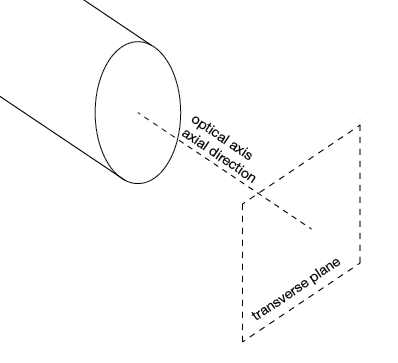
\includegraphics[width=0.4\textwidth]{Images/Background/axes.png}
% \caption{Definition of axes.\label{fig:axis_def}}
% \end{figure}

Throughout this document, the coordinate axis parallel to the direction of light emission from the objective shall be referred to as the ``axial'' direction, or ``z'' axis. The plane perpendicular to this axis is known as the ``transverse'' plane, or, sometimes, the ``x'' and ``y'' axes. %A diagram of this definition is shown in Figure~\ref{fig:axis_def}.

\begin{figure}[h!]
  \centering
    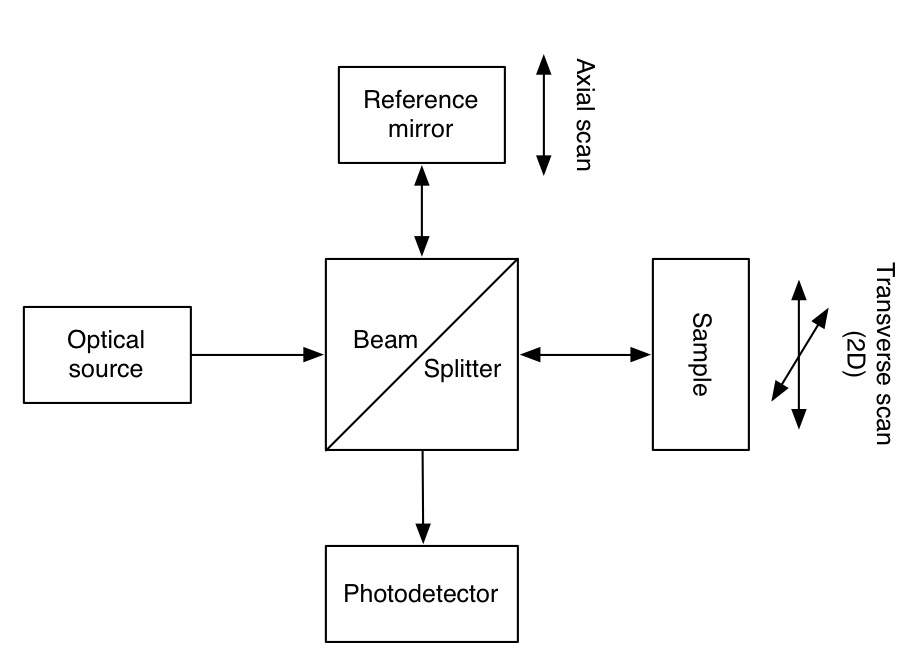
\includegraphics[width=0.75\textwidth]{Images/Background/basic_oct_2.png}
      \caption{Block diagram of a simplified OCT system.\label{fig:basic_oct}}
\end{figure}

OCT functions by utilizing the principle of the Michelson interferometer. A block diagram of a significantly simplified OCT system is shown in Figure~\ref{fig:basic_oct}. First, light is split into two beams. One beam is reflected from a mirror, and the other beam is scattered from a biological sample. The light is then recombined and the intensity measured by a photodetector. When the optical path lengths of the two beams are closely matched, an interference pattern may be observed. By using temporally incoherent (broadband) light, the interference pattern is capable of absolute localization, as will now be shown.

The electric field from a temporally incoherent source can be modeled accurately as a wide-sense stationary random process with a power spectral density (PSD) corresponding to the optical spectrum of the source \cite{bouma}. In the case where the scattering sample is replaced by a reflecting mirror, the mathematical analysis may be simplified greatly by assuming that the system is analyzing the interference of this random process with itself, delayed by the optical path length difference. With these assumptions, it is shown that the interference pattern is equivalent to the autocorrelation of the random process and may be related to the source PSD \cite{fercher}.

The intensity of light with analytic (complex) amplitude $V(t)$ is defined as

\begin{equation}
I(t) = |V(t)|^2 = V^*(t)V(t) \; .
\end{equation}

In an OCT system, the light from a reference path is combined with the light from a sample path after some delay. This may be expressed as

\begin{equation}
V_D(t; \Delta t) = V_S(t) + V_R(t + \Delta t) \; .
\end{equation}

As measuring instantaneous electric field amplitude is impossible, only the expected value, or the time average of the intensity, are of interest, indicated by the notation $\langle x(t) \rangle$. Letting $\Gamma_{XY}$ represent the cross correlation between two random processes $X$ and $Y$, the resulting intensity is

\begin{equation}
\begin{aligned}
\bar{I}_D(\Delta t) & =  \langle I_D(t; \Delta t) \rangle \\
& =  \langle V^*_D(t; \Delta t) V_D(t; \Delta t) \rangle \\
& =  \langle I_S(t) \rangle + \langle I_R(t) \rangle + 2 \operatorname{Re} (\Gamma_{SR} (\Delta t) ) \; .
\end{aligned}
\end{equation}

The time delay between the two signals, $\Delta t$, is proportional to the path length difference between the two beams, and may be calculated as $\Delta t = \Delta z / c$. When both the sample and reference paths are illuminated from the same light source, the cross correlation function above simplifies into an autocorrelation function of the light source. From here, the Wiener-Khinchin theorem can be applied, which states that the autocorrelation function of a wide-sense stationary random process is

\begin{equation}
\Gamma_{XX}(\tau) = 2 \int_{0}^\infty S_{XX}(f) \exp(2 \pi j \tau f) \,df
\end{equation}

\noindent straightforwardly related to the process power spectral density $S_{XX}(f)$ by a Fourier transform.

Therefore, the axial resolution in an OCT system is limited by the spectral properties of the light source. The width of the envelope of the autocorrelation function, and therefore the axial resolution, is found to be

\begin{equation} \label{eq:ares}
\delta_z = l_c = \frac{2 \ln{2}}{\pi} \frac{\lambda_0^2}{\Delta \lambda}
\end{equation}

\noindent for a source of center wavelength $\lambda_0$ and FWHM bandwidth $\Delta \lambda$, assuming a Gaussian PSD \cite{fercher}.

The autocorrelation function also has a periodic interference component, as the PSD $S_{XX}(f)$ in Equation~\ref{eq:ares} is not DC biased, but instead is centered around the central optical frequency of the source. In the spatial domain, this represents itself as a carrier wave modulating the autocorrelation envelope, with a spatial period of one wavelength. The time-domain frequency of this carrier as captured by the photodetector,

\begin{equation} \label{eq:carrier}
f_{mod} = 2 v_s / \lambda_0
\end{equation}

\noindent is therefore dependent both on the wavelength of the light source, $\lambda_0$, and the speed of the axial scan, $v_s$ \cite{fercher}. Note that the factor of two results from the fact that changing the length of the reference path by a distance $\Delta x$ changes the optical path length by $ 2 \Delta x$.

\subsection{Calculation of transverse resolution}
\label{sec:transverse_background}

The transverse resolution of the optical system is dependent on the optics used to shape and focus the light. In the case of the FO-DOCM system, these consist of an optical fiber, which projects light outward into the objective lens. The objective lens is a graded index (GRIN) lens, that uses glass with a continuously varying index of refraction to focus the light onto the desired focal point.

Light travels through a single mode fiber, and is emitted from a single mode fiber, as a Gaussian beam, a beam of light with a transverse intensity profile approximated by a Gaussian function. A Gaussian beam may also be described by a complex beam parameter $q$, more easily defined by its inverse

\begin{equation}
 \frac{1}{q(z)} = \frac{1}{R(z)} - i \frac{\lambda}{\pi w(z)^2}
 \label{eq:qparam}
 \end{equation}

\noindent where $R(z)$ is the radius of curvature, and $w(z)$ is the beam radius, defined as the point where intensity has fallen to $1/e^2$, at a distance $z$ from the beam waist \cite{Siegman}. Therefore, the beam radius may be found from the $q$ parameter by

\begin{equation}
 w(z) = \sqrt{\frac{-\lambda}{\pi \operatorname{Im} (1/q(z))}} \; .
 \label{eq:wz}
 \end{equation}

The transverse resolution is determined by the minimum spot size of the focused Gaussian beam of light. The evolution of a propagating Gaussian beam may be determined by matrices of the form

\begin{equation}
 \left( \begin{array}{cc}
a & b \\
c & d \end{array} \right)
\end{equation}

\noindent referred to as ABCD matrices, where

\begin{equation}
 q(z_2) = \frac{A q(z_1) + B}{C q(z_1) + D} \; .
 \label{eq:abcd_q}
 \end{equation}

The ABCD matrix for forward propagation through free space is

\begin{equation}
 \left( \begin{array}{cc}
1 & l \\
0 & 1 \end{array} \right)
\end{equation}

\noindent where $l$ is the distance traveled. The ABCD matrix for a graded index lens is

\begin{equation}
\left( \begin{array}{cc}
\cos{\sqrt{A} l} & (n_0 \sqrt{A})^{-1} \sin{\sqrt{A} l} \\
-(n_0 \sqrt{A}) \sin{\sqrt{A} l} & \cos{\sqrt{A} l} \end{array} \right)
\end{equation}

\noindent where the index profile of the GRIN lens is $n(r) = n_0 (1 - \frac{A r^2}{2})$, and the length of the lens is $l$ \cite{Siegman}.

Therefore, the cascaded transfer matrix for the entire system, from fiber emission to a focused spot, is 

\begin{equation}
\begin{aligned}
 & \left( \begin{array}{cc}
1 & l_1 \\
0 & 1 \end{array} \right)
\left( \begin{array}{cc}
\cos{\sqrt{A} l_2} & (n_0 \sqrt{A})^{-1} \sin{\sqrt{A} l_2} \\
-(n_0 \sqrt{A}) \sin{\sqrt{A} l_2} & \cos{\sqrt{A} l_2} \end{array} \right)
\left( \begin{array}{cc}
1 & l_3 \\
0 & 1 \end{array} \right) \\
= & 
\left(
\begin{array}{cc}
 \cos \left(\sqrt{A} l_2\right)-\sqrt{A} l_1 n_0 \sin
   \left(\sqrt{A} l_2 \right) & \frac{\sqrt{A} (l_1+ l_3)
   n_0 \cos \left(\sqrt{A} l_2 \right)+\left(1-A l_1 l_3
   n_0^2\right) \sin \left(\sqrt{A} l_2 \right)}{\sqrt{A} n_0}
   \\
 -\sqrt{A} n_0 \sin \left(\sqrt{A} l_2 \right) & \cos \left(\sqrt{A}
   l_2 \right)-\sqrt{A} l_3 n_0 \sin \left(\sqrt{A}
   l_2 \right) \\
\end{array}
\right)
\end{aligned}
\end{equation}

\noindent where $l_3$ is the distance from the end of the optical fiber to the GRIN lens, $l_2$ is the length of the GRIN lens, and $l_1$ is the distance from the end of the GRIN lens to the focal point. By applying Equation~\ref{eq:abcd_q}, the $q$ parameter of the focused beam is

\begin{equation}
q_1 = \frac{\sin (\sqrt{A} l_2) (A l_1 n_0^2
   (l_3+q_0)-1)-\sqrt{A} n_0 \cos (\sqrt{A}
   l_2) (l_1+l_3+q_0)}{A n_0^2 (l_3+q_0) \sin
   (\sqrt{A} l_2)-\sqrt{A} n_0 \cos (\sqrt{A}
   l_2)}
   \label{eq:q1}
\end{equation}

\noindent where $q_0$ is the $q$ parameter at emission. Using Equation~\ref{eq:wz}, and by multiplying by a scale factor, the beam radius can be converted to an expression for the transverse FWHM distance

\begin{equation}
\delta_x = \sqrt{2 \ln{2}} \sqrt{\frac{-\lambda}{\pi \operatorname{Im} (1/q_1)}}  \; .
\end{equation} 

% The transverse resolution limit is the standard diffraction limit for a lens, but, depending on the quality of the objective lens optics, this may not be achievable. In general, diffraction through a circular aperture creates an Airy distribution of light, with size dependent on the diameter of the aperture and its distance from the image. The FWHM size of the diffraction limited Airy disc is given as

% \begin{equation} \label{eq:tres}
% \delta_x = 0.51 \frac{\lambda_0}{\mathrm{NA}}
% \end{equation}

% \noindent where NA refers to the numerical aperture of the objective lens \cite{hecht}. In the paraxial approximation, the NA is equal to $D/(2f)$, where $f$ is the distance to the image, and $D$ is the aperture diameter.

\section{Heterodyne OCT with acousto-optic modulators}

As derived in the previous section, the speed of the z-axis motion defines the frequency of the interferogram carrier. For typical cases, this is on the order of 1 KHz. If the speed of the scan is variable, this carrier is inconsistent, and if the scan stops at a particular point, the frequency is near zero (non-zero only due to spurious mechanical vibration).

In some cases, such as when phase recovery of the carrier frequency signal is necessary, as is the case for the FO-DOCM system, it is desirable to have an independent carrier reference. This can also be useful for cases where the z-axis speed is zero, as in {\em en-face} OCT, or when a carrier frequency independent of the speed of the z-axis scan is desired. One method of accomplishing this is the use of an optical heterodyne, which may be created with acousto-optic modulators (AOMs), also known as Bragg cells \cite{bouma} \cite{hitzenberger}.

\subsection{Principle of operation of an AOM}

\begin{figure}[h!]
\centering
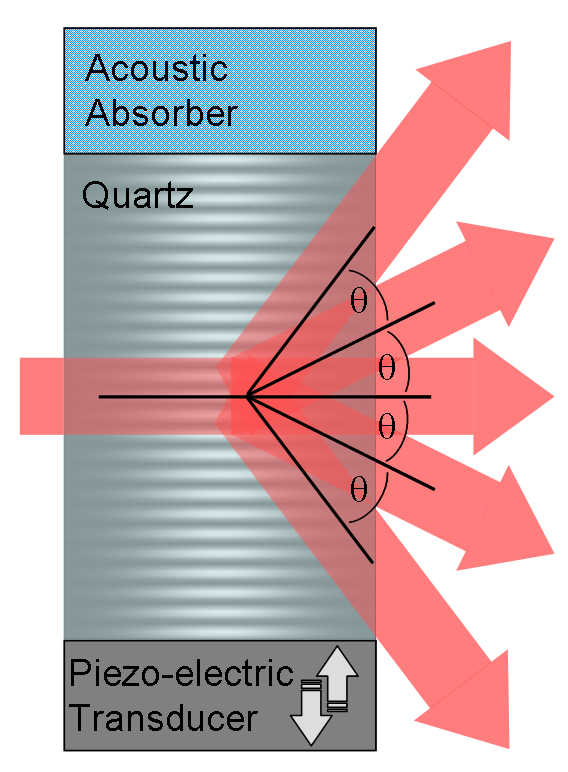
\includegraphics[width=0.3\textwidth]{Images/Background/aom.png}
\caption[Light scatters off of acoustic wavefronts in an acousto-optic modulator.]{Light scatters off of acoustic wavefronts in the quartz crystal of an acousto-optic modulator. As it scatters, it changes both frequency and angle. {\em Adapted from a public domain image by Jeff Lundeen.}}
\end{figure}

Acousto-optic modulators are crystals, typically quartz, that use the acousto-optic effect to shift the frequency of light. A transducer establishes an acoustic standing wave at radio frequencies, typically 40-200 MHz, inside the crystal. Acoustic compression waves in the crystal can be modeled as gradients in the refractive index. Light incident upon these refractive index gradients will be scattered, changing both angle and frequency. Momentum conservation of the scattered light requires

\begin{equation}
\mathbf{k}_{\mathrm{acoustic}} + \mathbf{k}_{\mathrm{incident}} = \mathbf{k}_{\mathrm{diffracted}}
\end{equation}

\noindent be satisfied by the wave vectors of the acoustic, incident optical, and diffracted optical waves \cite{haus}.

This can be solved to give a condition on the angle in the case where $\mathbf{k}_i$ is orthogonal to $\mathbf{k}_s$,

\begin{equation} 
\sin{\theta} \approx \frac{|\mathbf{k}_s|}{|\mathbf{k}_i|} = \frac{\lambda}{n\Lambda}
\end{equation}

\noindent with optical wavelength $\lambda$ and acoustic wavelength $\Lambda$. A small angle approximation is applied as it is assumed that $|\mathbf{k}_i| \gg |\mathbf{k}_s|$.

In some crystals, higher order diffraction angles occur, however, it is difficult to achieve high modulation efficiencies, and they are not of significant interest to this research.

% \begin{figure}[h!]
% \centering
% 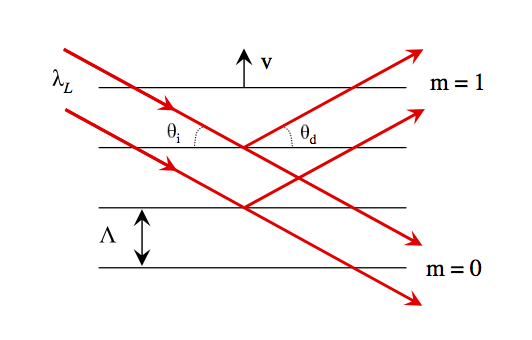
\includegraphics[width=0.5\textwidth]{Images/Background/aom_scattering.png}
% \caption{Light scattering off of acoustic wavefronts in an acousto-optic modulator.}
% \end{figure}

% Scattered light interferes constructively when the following condition is met.

% \begin{equation} \label{eq:constructive_interference}
% n \lambda_L = \Lambda (\sin{\theta_i} + \sin{\theta_d})
% \end{equation}

% Conservation of momentum requires that $\theta_i = \theta_d$, which simplifies the constructive interference condition to:

% \begin{equation}
% n \lambda_L = 2 \Lambda \sin{\theta_d}
% \end{equation}

Energy conservation further requires that the frequency of scattered light be shifted by $F$, the acoustic wave frequency \cite{haus}. This frequency shift is what makes an AOM of practical interest for optical heterodyning.

\subsection{Generating a carrier wave with an AOM}
\label{sec:aom_carrier}

Even with an imprecise or drifting optical center frequency, the precise shift frequency induced by an AOM can be used to generate an extremely stable optical interference signal \cite{hitzenberger}. 

The instantaneous complex electric fields for monochromatic plane waves in a particular location of two different frequencies, $f$ and $f + F$, may be written as

\begin{equation}
\begin{aligned}
E_a(t) & = E_a \exp{(2 \pi ft j)} \\
E_b(t) & = E_b \exp{(2 \pi (f + F)t j)} \; .
\label{eq:complex_field_amplitudes}
\end{aligned}
\end{equation}

The interference between the superposition of these two fields,

\begin{equation}
\begin{aligned}
E_a(t) + E_b(t) = & E_a \exp{(2 \pi ftj)} + E_b \exp{(2 \pi (f + F)t j)} \\
= & E_a \exp{(2 \pi ftj)} + E_b (\exp{(2 \pi ftj)} \exp{(2 \pi Ftj)}) \\
= & E_a \exp{(2 \pi ftj)} (1 + \frac{E_b}{E_a} \exp{(2 \pi Ftj)}) \\
= & E_a(t) (1 + \frac{E_b}{E_a} \exp{(2 \pi Ftj)})
\end{aligned}
\end{equation}

\noindent creates a beat frequency, with the amplitude of the optical frequency modulated by the slower, and detectable RF frequency $F$.

For many applications, the radio frequency $F$ used to drive the AOMs is a higher frequency carrier than is desired. In this case, it is possible to use two AOMs to generate an even lower frequency carrier by driving them each at slightly different RF frequencies, resulting in complex field amplitudes 

\begin{equation}
\begin{aligned}
E_a(t) & = E_a \exp{(2 \pi t j (f + F_1))} \\
E_b(t) & = E_b \exp{(2 \pi t j (f + F_2))} \; .
\end{aligned}
\end{equation}

It can be seen via an identical simplification to the above that the combination of these electric field amplitudes creates a carrier wave with frequency equal to the absolute value of $F_1 - F_2$.

\section{Doppler OCT with AOMs}
\label{sec:Doppler_aom}

%% more equations/background

Optical scattering from moving particles also induces a change in the frequency of scattered light due to the Doppler effect. This change in frequency can be expressed as

%Because the speed of scattering media will always be much smaller than the speed of the light, the change in frequency caused by the Doppler effect is:

\begin{equation} \Delta f(t) = 2 \frac{v(t)}{c} f_0 \cos{(\beta)} \sin{(\frac{\alpha}{2})} \end{equation}

\noindent where $\alpha$ is the angle between the direction of incident light propagation and the  light detector, $\beta$ is the angle between the direction of light propagation and the direction of motion of the media, and $v(t)$ is the instantaneous velocity of the sample \cite{hurst}.

In the FO-DOCM apparatus, only backscattered light can be detected, so $\alpha$ is assumed to be $\pi$ radians. The direction of motion is assumed to be in the direction of light propagation for simplicity, so that $\beta = 0$. The equation for the instantaneous frequency change then simplifies to

\begin{equation} \Delta f(t) = 2 \frac{v(t)}{c} f_0 \end{equation}

Integrating the instantaneous frequency finds the phase, up to a constant term, as

\begin{equation}
\begin{aligned}
\phi(t) & = \int 2 \pi f(t) \mathrm{d}t \\
& = 2 \pi \int f_0 (1 + 2 \frac{v(t)}{c}) \mathrm{d}t \\
& = 2 \pi \left( f_0 t + 2 \frac{d(t)}{c} \right)
\end{aligned}
\end{equation}

\noindent where $d(t)$ is the instantaneous sample displacement, the integral of the sample velocity.

In an analogous way to Equation~\ref{eq:complex_field_amplitudes}, instantaneous field amplitudes $E_a$ and $E_b$, representing the sample and reference paths respectively, may be written as

\begin{equation}
\begin{aligned}
E_a(t) & = E_a \exp{\left(2 \pi j (f + 2 F_1) \left( t + 2 \frac{d(t)}{c}\right) \right)}  \\
E_b(t) & = E_b \exp{(2 \pi t j (f + 2 F_2))}
\end{aligned}
\end{equation}

\noindent where $E_a$ has scattered from media moving with velocity $v(t)$ and has passed through an AOM of frequency $F_1$, while $E_b$ has been reflected from a stationary object and has passed through an AOM of frequency $F_1$. Note that the radio frequencies $F_1$ and $F_2$ have been multiplied by two, as light must make two passes through each AOM.

The electric field at the detector is the sum of the two electric field amplitudes,

\begin{dmath}
E_b(t) + E_a(t) = E_a \exp{(2 \pi t j (f + 2 F_1))}\left(\exp{\left(2 \pi j \frac{2 d(t)}{c}(f + 2 F_1)\right)} + \frac{E_b}{E_a} \exp{(2 \pi t j 2 (F_2 - F_1))}\right) \; .
\end{dmath}

This equation may be simplified slightly by substituting two new symbols for the modified optical frequency, $f' = f + 2 F_1$, and radio frequency difference, $\Delta F = F_2 - F_1$, to

\begin{dmath}
E_b(t) + E_a(t) = E_a \exp{(2 \pi t j f')}\left(\exp{\left(2 \pi j f' \frac{ 2 d(t)}{c}\right)} + \frac{E_b}{E_a} \exp{(-2 \pi t j 2 \Delta F)}\right) \; .
\end{dmath}

The instantaneous light intensity is equivalent to the absolute value of the instantaneous electric field amplitude squared, given by

% \begin{dmath}
% I(t) = E_a^2 \left(1 + \frac{E_b^2}{E_a^2} + 2 \frac{E_b}{E_a} \cos{\left(2 \pi t \left(\Delta F + f' \left( \frac{2 A_o \cos{\omega t}}{c} \right) \right)\right)} \right)
% \end{dmath}

\begin{dmath}
I(t) = E_a^2 + E_b^2 + 2 E_b E_a \cos{ 2 \pi \left(2 t \Delta F + f' \frac{2 d(t)}{c}   \right)} \; .
\end{dmath}

The result of the frequency shift induced by the motion of the media can clearly be seen in the instantaneous phase of the intensity oscillation,

\begin{dmath}
\label{eq:phase_aom_Doppler}
\phi(t) = 2 \pi \left(2 t \Delta F + f' \frac{2 d(t)}{c}   \right) \; .
\end{dmath}

This is equivalent to phase modulation, with the periodic change in phase of

\begin{equation}
2 \pi f' \left( \frac{2 d(t)}{c} \right) \; .
\end{equation}

This oscillation can be extracted from the captured signal using the Hilbert transform, discussed in Section \ref{sec:sigproc_mo_anal}. While this derivation assumed perfectly monochromatic light sources, as would be the case in an ideal laser interferometer, the result generalizes to the non-monochromatic random signals used in Section~\ref{sec:principles_oct}.

\section{Signal processing}

%% signal processing figure

\begin{figure}[h!]
  \centering
  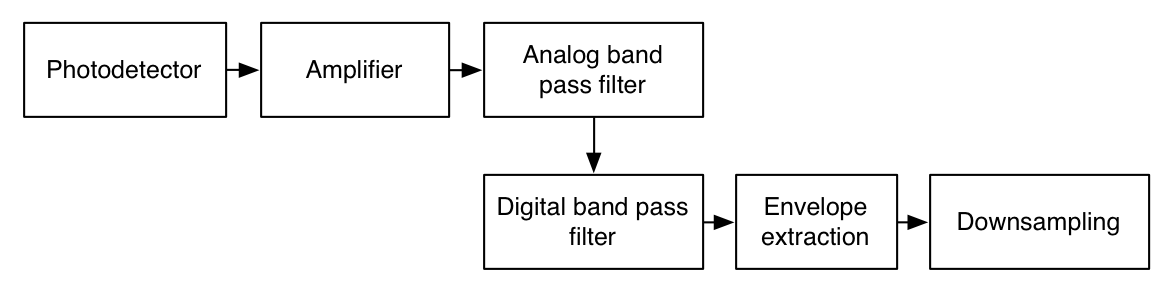
\includegraphics[width=1.0\textwidth]{Images/background/basic_dsp.png}
% \begin{tikzpicture}[node distance = 2cm, auto]
%     % Place nodes
%     \node [block] (bpf) {Analog band pass filter and preamplifier};
%     \node [block, left of=bpf, node distance=3cm] (pd) {Photodiode};
%     \node [block, right of=bpf, node distance=3cm] (adc) {Analog to digital converter};
%     \node [block, below of=adc, node distance=3cm] (dbpf) {Digital band pass filter};
%     \node [block, right of=dbpf, node distance=3cm] (hilb) {Hilbert transform envelope extraction};
%     \node [block, right of=hilb, node distance=3cm] (ds) {Downsampling};
%     % Draw edges
%     \path [line] (pd) -- (bpf);
%     \path [line] (bpf) -- (adc);
%     \path [line] (adc) -- (dbpf);
%     \path [line] (dbpf) -- (hilb);
%     \path [line] (hilb) -- (ds);
% \end{tikzpicture}
\caption[Basic OCT signal processing chain.]{Basic OCT signal processing chain. The bandpass filter is centered around the carrier frequency from equation \ref{eq:carrier}. The demodulator can be either as straightforward as an envelope follower or a Hilbert transform based analytic continuation.}
\end{figure}

After detection and amplification, but prior to analog-to-digital conversion, analog bandpass filters select for the carrier frequency and its sidebands, in addition to bandlimiting the signal below the Nyquist frequency. The signal is then sampled and quantized by an ADC so that it may be manipulated digitally.

The Hilbert transform can then be used to extract the envelope from the modulated carrier signal. Assuming a signal of the following form, 

\begin{equation}
x(t) = A(t)\cos{(\omega t)}
\end{equation}

\noindent the Hilbert transform can generate the approximate quadrature component,

\begin{equation}
H(x(t)) \approx A(t) \sin{(\omega t)} \;
\end{equation}

where $A(t)$ is a real envelope \cite{oppenheim}.

It can therefore be seen that the envelope component of the signal can be calculated as 

\begin{equation}
A(t) \approx \sqrt{(x(t))^2 + H(x(t))^2} \; .
\end{equation}

The envelope, which does need the high sampling rate previously required in order to capture the carrier frequency, can then be low pass filtered and decimated to the resolution required by the imaging application.

Additionally, it can be seen that the instantaneous phase of this arbitrary sinusoidal signal may also be estimated using the Hilbert transform as

\begin{equation}
\phi(t) \approx \tan^{-1} \left( \frac{H(x(t))}{x(t)} \right) \; .
\label{eq:hilbert_phase}
\end{equation}

\subsection{Analyzing motion}
\label{sec:sigproc_mo_anal}

%As the reference signal $V_{ref}$ is at exactly half the frequency of the captured heterodyne signal $V_{het}$, the following equation gives the instantaneous difference in phase.

As shown in Section \ref{sec:Doppler_aom}, the phase of the intensity of light scattered from moving media, referred to as the heterodyne phase, $\phi_{\mathrm{het}}$, can be expressed as

\begin{equation}
\phi_{\mathrm{het}}(t) = 2 \pi \left(2 t \Delta F + f'  \frac{2 d(t)}{c}    \right) \; .
\end{equation}

A reference signal must also be captured, which oscillates at a frequency equal to the difference of the two RF drive frequencies. The phase of this difference is

\begin{equation}
\phi_{\mathrm{ref}}(t) = 2 \pi t \Delta F
\end{equation}

\noindent exactly half the phase of the carrier frequency of the heterodyne signal.

Subtracting twice the reference phase from the heterodyne phase, and replacing $c$ by $c/n$ to account for the refractive index of the media, finds the phase difference

\begin{equation}
\phi_{\mathrm{dif}}(t) = \phi_{\mathrm{het}}(t) - 2 \phi_{\mathrm{ref}}(t) = 2 \pi f' \left( \frac{2 d(t)}{c/n} \right) \; .
\end{equation}

Because the RF frequency $F_1 << f$, the optical frequency, it may be approximated as $f' = f + F_1 \approx f$, simplifying the equation above. Expressing the optical frequency as a wavenumber further simplifies the phase difference to % TO DO DEFINE K 5/13

\begin{equation}
\phi_{\mathrm{dif}}(t) = 2 \pi t f'  \left( \frac{2 d(t)}{c/n} \right) \approx 2 k n d(t) \; .
\label{eq:phi_diff}
\end{equation}

Using the result from Equation~\ref{eq:hilbert_phase}, the instantaneous phase difference between the captured heterodyne signal, $V_{\mathrm{het}}$, and the captured reference signal $V_{\mathrm{ref}}$, may be written as

\begin{equation}
\phi_{\mathrm{dif}}(t) \approx \tan^{-1}\left( \frac{H(V_{\mathrm{het}}(t))}{V_{\mathrm{het}}(t)} \right) - 2\tan^{-1}\left( \frac{H(V_{\mathrm{ref}}(t))}{V_{\mathrm{ref}}(t)} \right) \; .
\label{eq:phi_diff2}
\end{equation}

Combining Equations~\ref{eq:phi_diff} and \ref{eq:phi_diff2}, the periodic displacement of the sample may be calculated as

\begin{equation}
\begin{aligned}
 %d(t)  & \approx \frac{1}{2kn} \phi_{\mathrm{dif}}(t) \\
 d(t)  & \approx \frac{1}{2kn} \left( \tan^{-1}\left( \frac{H(V_{\mathrm{het}})(t)}{V_{\mathrm{het}}(t)} \right) - 2\tan^{-1}\left( \frac{H(V_{\mathrm{ref}})(t)}{V_{\mathrm{ref}}(t)} \right) \right) \; .
%&  \approx \frac{1}{2kn} \left( \tan^{-1}\left( \frac{H(V_{\mathrm{het}})(t)}{V_{\mathrm{het}}(t)} \right) - 2\tan^{-1}\left( \frac{H(V_{\mathrm{ref}})(t)}{V_{\mathrm{ref}}(t)} \right) \right)
\end{aligned}
\end{equation}

\section{Related work}

Since the 1960s, interferometry with laser light has been used to measure vibration in the cochlea. Early laser Doppler interferometer experiments required the placement of reflective beads to isolate tissues of interest; however, these beads can influence the mechanical properties of the cochlea~\cite{Nuttall2012}. Recent methods involving laser Doppler interferometry have had success in measuring vibrations with a noise floor as low as 30 pm/Hz$^{0.5}$ without beads, but also require a parallel system, such as confocal microscopy, in order to produce an image of the tissues \cite{Jacob2009} \cite{Ren2002} \cite{Ren2011} . Furthermore, laser interferometers are highly coherent, so without reflective beads, vibration measurements have a depth separation determined primarily by the beam divergence angle, resulting in poor axial isolation.

Low coherence interferometry, such as OCT, is capable of solving these problems. As mentioned in Section \ref{sec:intro}, this FO-DOCM system is designed to update the previous free space system used in the Micromechanics Group. The FO-DOCM system is quite similar to the FS-DOCM system, but is also different in several ways: the use of fiber optic components rather than free space optics, the use of a longer wavelength source, and the revised alignment and positioning apparatus  \cite{hong}. Furthermore, the FO-DOCM system allows for continuous scanning of lines in an image in addition to point-by-point pixel acquisition.

\paragraph{Other time-domain Doppler OCT systems.} The use of acousto-optic modulators is not essential for Doppler OCT, and systems similar to the FO-DOCM system have been constructed without them. However, without a reference signal to use in extracting phase modulation information, the system responds to vibration amplitude in a very non-linear way. Furthermore, because vibrations are not modulated to higher frequencies by the heterodyne carrier, more interference at low frequencies, from mechanical vibrations and electrical $1/f$ noise, results in a higher noise floor, typically on the order of 30 pm/Hz$^{0.5}$ \cite{Choudhury2006}.

\paragraph{Spectral-domain Doppler OCT systems.} While the FO-DOCM project uses time-domain Doppler OCT, work has also been done in the field of spectral domain Doppler OCT. Spectral-domain Doppler OCT systems have achieved results with an axial resolution of 13 \micron~and a motion detection noise floor of 300 pm/Hz$^{0.5}$ \cite{Choudhury2011} \cite{Subhash2012}. It is thought that a time domain approach can result in higher resolution motion measurements than a spectral domain system, as monolithic photodiodes have better noise equivalent power than a CCD line camera with a diffraction grating. Furthermore, the sampling rate of a CCD sensor is very limited compared to a photodiode, restricting the speed and accuracy of phase recovery. However, the use of a time-domain system adds the considerable expense of requiring physical motion to scan the z-axis, resulting in significantly slower image acquisition.

\paragraph{Trans-bone imaging.} Doppler OCT has been previously used with some success for measuring vibrations of cochlear tissues through bone. Using a 935 nm center wavelength, motion inside an {\em in vivo} mouse cochlea was measured with an noise floor of approximately 100 pm/Hz$^{0.5}$ \cite{Gao2013}. It is suspected that a 1310 nm center wavelength, as used in the FO-DOCM system, will be even more effective at penetrating bony tissue \cite{Sandell2011} \cite{Bashkatov2006}. 

\paragraph{Microangiography.} Doppler OCT is not restricted to measuring periodic vibrations -- one of its first applications was for angiography, measuring the velocity of blood flow inside tissue. Current techniques with Doppler optical microangiography are capable of isolating and measuring blood flow in a single vessel over time  \cite{Dziennis2012}. While low frequency motion measurements such as constant motion have a significantly higher noise floor, blood flow velocity amplitudes are also typically much greater than vibrational amplitudes.

%\subsection{Positioning and GRIN lens}

\paragraph{Miniaturization of OCT apparatus} One of the advantages of the FO-DOCM system to the Micromechanics Group is its smaller size, so this work may be seen as continuing the active effort of minimizing the size of the OCT apparatus. Research in this area includes the creation of a miniature swept frequency laser source for OCT imaging \cite{Goldberg2009}, which could enable a higher axial resolution in a smaller form factor. GRIN lenses, used in the FO-DOCM system, have a significant size advantage in addition to high quality optical performance and have also been used in previous research as endoscopic probes for OCT \cite{Xie2006}.

% talk about uniqueness of our mechanical apparatus?

% small size is relevant here???


% ====================================

% 

% %Why time domain? This differentiates our work? Can I spin it positively?

% \cite{Choudhury2011}  % The FO-DOCM system is shown to be competitive with these results. \cite{Choudhury2011} \cite{Subhash2012}


% Also of interest in the development of this system, and still a developing technique, is the use of algorithms and more sophisticated signal processing techniques to improve the image quality and resolution ability of captured OCT data. Of significant interest is the possibility of correcting for dispersive effects caused by the propogation of light through the sample media. \cite{Xie2005} \cite{DrexlerBook} These techniques could also potentially be used to correct for dispersion caused by fiber length mismatch between the reference and sample paths, as discussed in Section~\ref{sec:reference_path}.

\paragraph{} Overall, the FO-DOCM system designed and constructed in this thesis builds on previous work and ideas in optical coherence tomography to develop an apparatus that satisfies the unique set of requirements of the Micromechanics Group, with advantages in motion resolution, tissue penetration, mechanical adjustability, and size.